\vfill 
\chapter{Conception}
\label{chap:conception}
\mtcaddchapter
\section*{Introduction}
\justifying
Dans ce chapitre, nous allons nous concentrer sur la conception de notre application en détail. Tout d'abord, nous présenterons l'architecture globale de l'application suivie de la conception de la base de données. Ensuite, nous présenterons la conception détaillée qui comprendra les vues statiques illustrées à l'aide de diagrammes de classes ainsi que les vues dynamiques illustrées à l'aide d'une variété de diagrammes telle que les diagrammes de séquence de conception, diagramme d’activité, diagramme d’états-transitions et diagramme de timing. Enfin, nous ferons quelques maquettes pour la conception graphique.

\section{Modèle architectural}
\justifying
Avant de démarrer la conception de notre application, il est essentiel de déterminer le modèle architectural qui répondra le mieux à nos besoins. Dans le cas de notre application, nous avons choisi d'adopter l'architecture 3-tiers ainsi que le modèle de conception \textbf{M}odèle-\textbf{V}ue-\textbf{C}ontrôleur \textbf{(MVC)}.

\subsection{Architecture physique (Architecture 3-tiers)}
\justifying
Notre plateforme sera mise en place physiquement selon l’architecture 3-tiers. Cette dernière, illustrée par la Figure 4.1, est constituée de trois couches distinctes: la couche de présentation, la couche logique de l'application et la couche de stockage des données.
\begin{itemize}[itemsep=1pt, parsep=1pt]
    \item \textbf{La couche de présentation : }Cette couche est chargée d'afficher les données et d'interagir avec l'utilisateur. Elle peut être intégrée à l'aide d'un navigateur web pour une application web.
    \item \textbf{La couche de logique de l’application : }Cette couche contient la logique métier de l'application. Les opérations de l'application sont gérées par cette couche comme la validation des données, la logique d'authentification, la gestion des erreurs et etc.
    \item  \textbf{La couche de stockage de données : } Cette couche occupe la position la plus basse. Elle gère les données de l'application. Cette couche peut être constituée d’un ou plusieurs bases de données, de services web ou de toute autre source de données.
\end{itemize}

\begin{figure}[H]
    \centering
    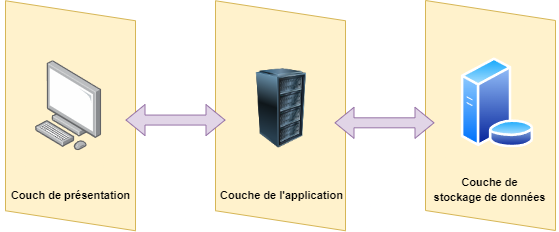
\includegraphics[width=\textwidth]{images/chp4/fig1.png}
    \caption{L’architecture 3-tiers}
    \label{fig:architecture-3-tiers}    
\end{figure}

L'architecture à 3 couches est adoptée grâce à sa capacité de  séparer, clairement, les différentes fonctionnalités de l'application et sa clarté dans la distinction entre les différentes couches. En outre, cette approche facilite la maintenance, l'évolutivité et la réutilisation du code.

\subsection{Architecture logique (Modèle MVC)}
Notre plateforme est structurée, logiquement, selon le patron architectural MVC (Model-View-Controller). Ce dernier est un modèle de conception utilisé pour les applications logicielles qui divise les diverses responsabilités de l'application en trois éléments distincts :
\begin{itemize}[itemsep=1pt, parsep=1pt]
    \item \textbf{Le Modèle (Model) : }Il symbolise le niveau de données de l'application. Il gère la logique métier et les échanges avec la base de données ou les services externes.
    \item \textbf{La Vue (View) : }Elle présente la partie de présentation de l’application. Elle a pour but de présenter visuellement les données et d’interagir avec l’utilisateur.
    \item  \textbf{Le Contrôleur (Controller) : }Il présente le niveau de contrôle de l'application. Son rôle consiste à gérer les interactions des utilisateurs et à orchestrer les actions à réaliser. Le contrôleur établit une communication avec le modèle afin de récupérer ou de mettre à jour les données ainsi qu'avec la vue pour visualiser les résultats.
\end{itemize}
La Figure 4.2 illustre le modèle MVC.
\begin{figure}[H]
    \centering
    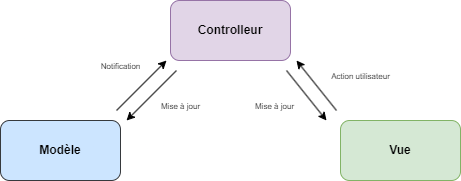
\includegraphics[width=0.8\textwidth,height=0.4\textwidth]{images/chp4/fig2.png}
    \caption{L’architecture du modèle MVC}
    \label{fig:architecture-MVC}    
\end{figure}
\noindent Ce choix est fait parce que le modèle MVC offre plusieurs avantages pour la conception et la maintenance d'applications logicielles. Tout d'abord, il permet une séparation claire des préoccupations qui facilite la gestion du code et la réutilisation des composants. En divisant les responsabilités de l'application en trois éléments distincts, chaque élément peut être développé et testé de manière autonome pour simplifier la collaboration et la gestion du code.

\subsection{Architecture applicative}
Dans notre architecture, nous avons divisé les différentes parties en fonction des serveurs utilisés. Voici les différentes parties de notre architecture :
\begin{itemize}[itemsep=1pt, parsep=1pt]
    \item \textbf{La couche de présentation (Navigateur) : }Il s'agit de l'endroit où l'application Next.js s'exécute dans le navigateur de l'utilisateur.
    \item \textbf{La couche de logiciel de l'application : }Cette couche a été divisée en 2 parties.
        \begin{itemize}[itemsep=1pt, parsep=1pt]
            \item \textbf{Runtime Node.js :}Il s'agit de l'endroit où le code Next.js côté serveur s'exécute sur un serveur Node.js.
            \item \textbf{Runtime Edge :}Il s'agit de l'endroit où les fonctions Vercel Edge s'exécutent sur un serveur dédié aux fonctions Edge.
        \end{itemize}
    \item  \textbf{La couche de stockage de données : }Cette couche a été divisée en 3 parties.
    \begin{itemize}[itemsep=1pt, parsep=1pt]
        \item \textbf{Postgres :}Il s'agit de l'endroit où la base de données Supabase Postgres réside sur un serveur dédié à la base de données.
        \item \textbf{Stockage :}Il s'agit de l'endroit où le stockage Supabase réside sur un serveur AWS dédié au stockage.
        \item  \textbf{Base de données vectorielles :}Il s'agit de l'endroit où la base de données vectorielles Pinecone réside sur un serveur dédié à la base de données vectorielles.
    \end{itemize}
\end{itemize}
En divisant notre structure en fonction des serveurs utilisés, nous avons réussi à séparer les différentes parties de l'application en les divisant en tiers puis en subdivisant chaque niveau en serveurs. De cette façon, chaque serveur peut être administré de manière autonome qui permet aux développeurs de se focaliser sur leur domaine de spécialisation respectif pour simplifier la maintenance, l'évolution et la réutilisation du code.\\
Dans la Figure 4.3, nous représentons l’architecture globale de notre plateforme.

\begin{figure}[H]
    \centering
    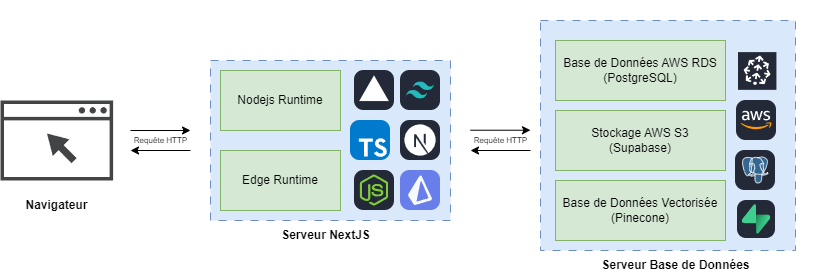
\includegraphics[width=1.15\textwidth, height=0.5\textwidth]{images/chp4/fig3.png}
    \caption{L’architecture applicative}
    \label{fig:architecture-applicative}    
\end{figure}

\subsection{Déploiement de notre plateforme}
Pour représenter le déploiement de notre plateforme, nous avons utilisé le diagramme de déploiement (voir Figure 4.4). Ce diagramme est une vue statique qui illustre l'utilisation de l'infrastructure physique par le système ainsi que la  répartition des composants du système et les relations entre eux.
\begin{figure}[H]
    \centering
    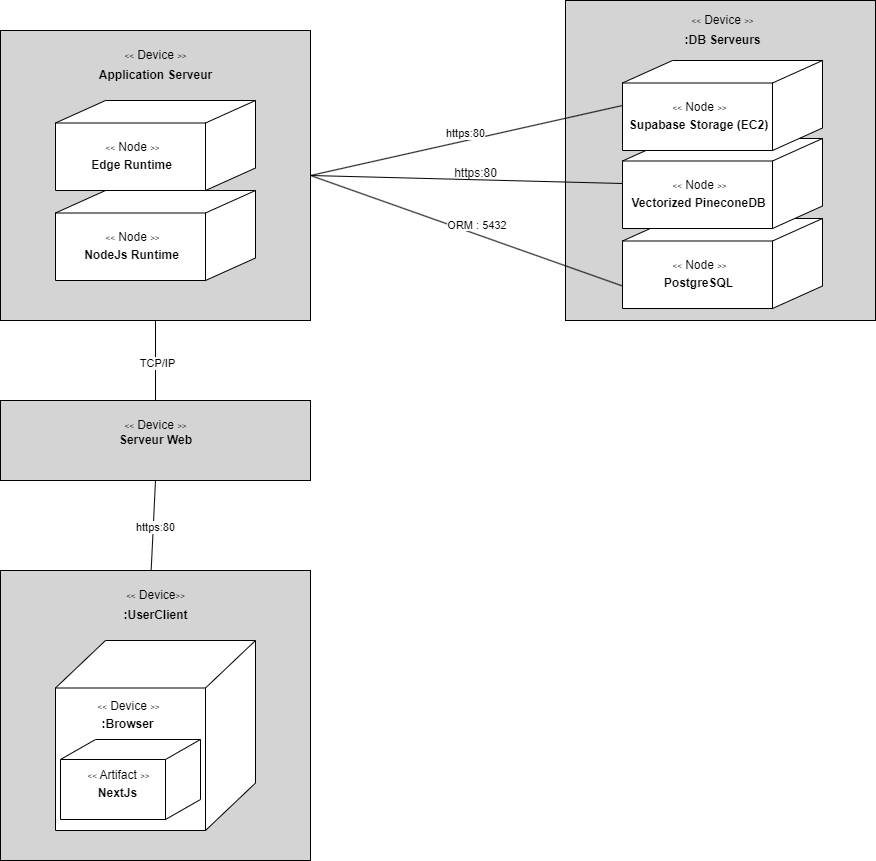
\includegraphics[width=\textwidth,height=0.8\textwidth]{images/chp4/fig4.png}
    \caption{Diagramme de déploiement de notre plateforme}
    \label{fig:Diagramme de déploiement de notre plateforme}    
\end{figure}

\section{Conception de la base de donnée}
\justifying
La conception d'une base de données implique de structurer les données selon un modèle spécifique qui définit leur organisation, leur stockage et leurs relations. Dans cette optique, nous débuterons par la présentation du \textbf{m}odèle \textbf{c}onceptuel de \textbf{d}onnées \textbf{(MCD)}. Ensuite, nous nous tournerons vers le \textbf{m}odèle \textbf{l}ogique de \textbf{d}onnées \textbf{(MLD)}.

\subsection{Modèle conceptuel de données}
Un modèle conceptuel de données permet de représenter les entités et les relations entre elles dans un système d’information.\\
La Figure 4.5 illustre le modèle conceptuel de notre application.
\begin{figure}[H]
    \centering
    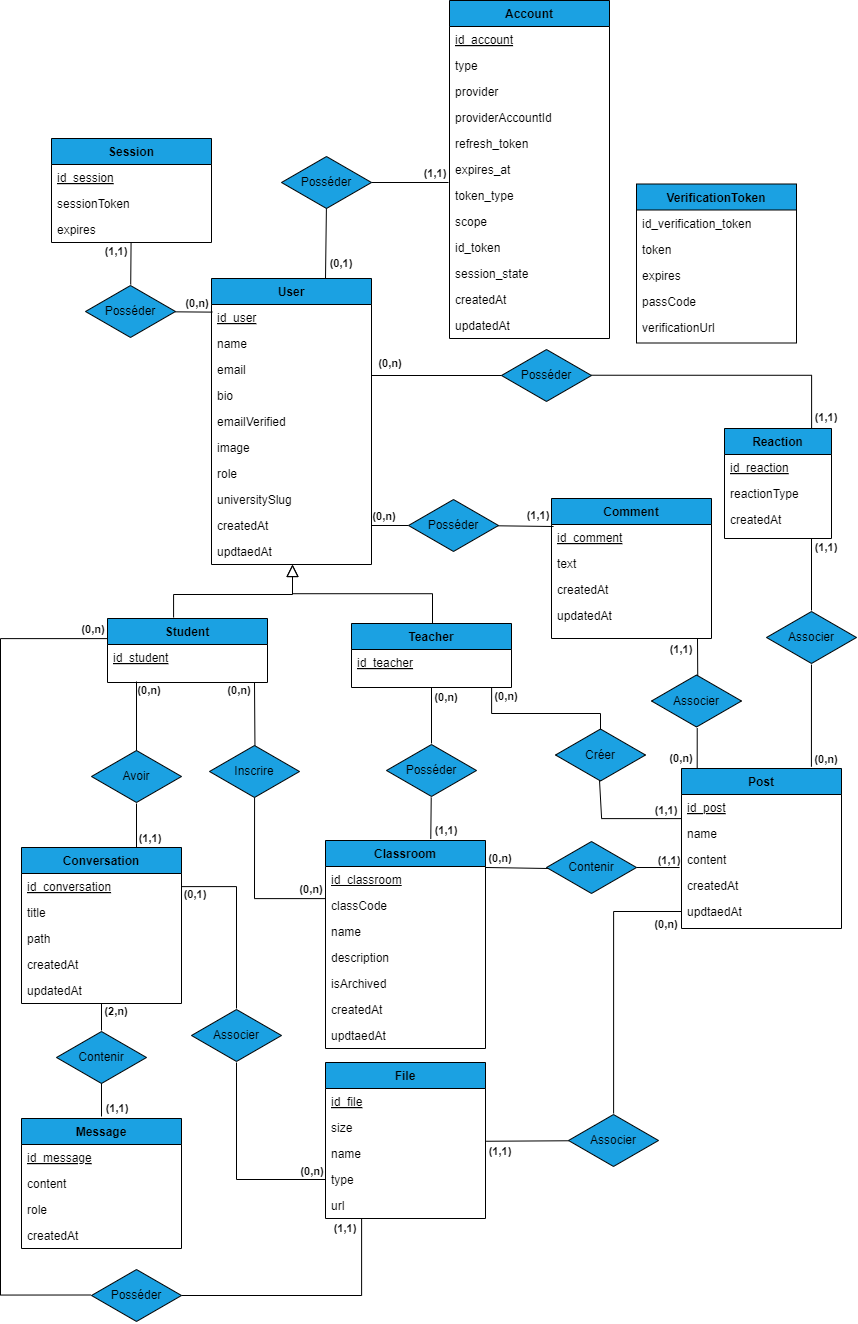
\includegraphics[width=1.1\textwidth,height=1.4\textwidth]{images/chp4/fig5.png}
    \caption{Modèle conceptuel de données (MCD)}
    \label{fig:Modèle conceptuel de données (MCD)}    
\end{figure}


\subsection{Modèle logique de données}
Pour organiser un modèle MCD, différents modèles logiques de données peuvent être utilisés. Dans notre projet, nous avons choisi d'utiliser le modèle relationnel car il répond bien à nos besoins non fonctionnels. En suivant les règles de transformation du modèle entité-association vers un modèle relationnel, nous obtiendrons le schéma relationnel suivant : \\
\textbf{Account} ( \textbf{\uline{id\_account}} , type , provider , providerAccountId , refresh\_token , access\_token , expires\_at , token\_type , scope , id\_token , session\_state , createdAt , updatedAt , \#id\_user ) \\
\textbf{Session} ( \textbf{\uline{id\_session}} , sessionToken , expires , \#id\_user ) \\ 
\textbf{User} ( \textbf{\uline{id\_user}} , name , email , bio , emailVerified , image , rôle , universitySlug , createdAt , updatedAt ) \\
\textbf{VerificationToken} ( \textbf{\uline{id\_verification\_token}} , token , expires , passCode , verificationUrl ) \\
\textbf{Teacher} ( \textbf{\uline{id\_teacher}} , \#id\_user ) \\
\textbf{Student} ( \textbf{\uline{id\_student}} , \#id\_user ) \\
\textbf{Classroom} ( \textbf{\uline{id\_classroom}} , classCode , name , description , isArchived , createdAt , updatedAt , \#id\_teacher ) \\
\textbf{Post} ( \textbf{\uline{id\_post}} , name , content , createdAt , updatedAt , \#id\_teacher , \#id\_classroom) \\
\textbf{File} ( \textbf{\uline{id\_file}} , size , name , type , url , \#id\_post , \#id\_student ) \\
\textbf{Comment} ( \textbf{\uline{id\_comment}}, text, createdAt , updatedAt , \#id\_user , \#id\_post ) \\
\textbf{Reaction} ( \textbf{\uline{id\_reaction}} , reactionType , createdAt , \#id\_user , \#id\_post ) \\
\textbf{Conversation} ( \textbf{\uline{id\_conversation}} , title , path , createdAt , updatedAt , \#id\_student , \#id\_file ) \\
\textbf{Message} ( \textbf{\uline{id\_message}} , content , role , createdAt , \#id\_conversation ) \\
\textbf{Inscrire} ( \uline{\textbf{\#id\_student} , \textbf{\#id\_classroom}} )

\section{Conception Logicielle}
Dans cette section, nous allons réaliser une conception détaillée de notre application de point de vue statique et dynamique.

\subsection{Conception de la vue statique: Diagramme de classes}
Les diagrammes de classes sont des représentations statiques et structurelles utilisées pour présenter les classes, les interfaces et leurs relations dans un système logiciel. En effet, les diagrammes de classes sont une partie importante de la conception détaillée d'un système logiciel car ils permettent de présenter visuellement la structure du système et les interactions entre ses différents composants.\\
La Figure 4.6 illustre le diagramme de classes d’analyse de notre plateforme.

\begin{figure}[H]
    \centering
    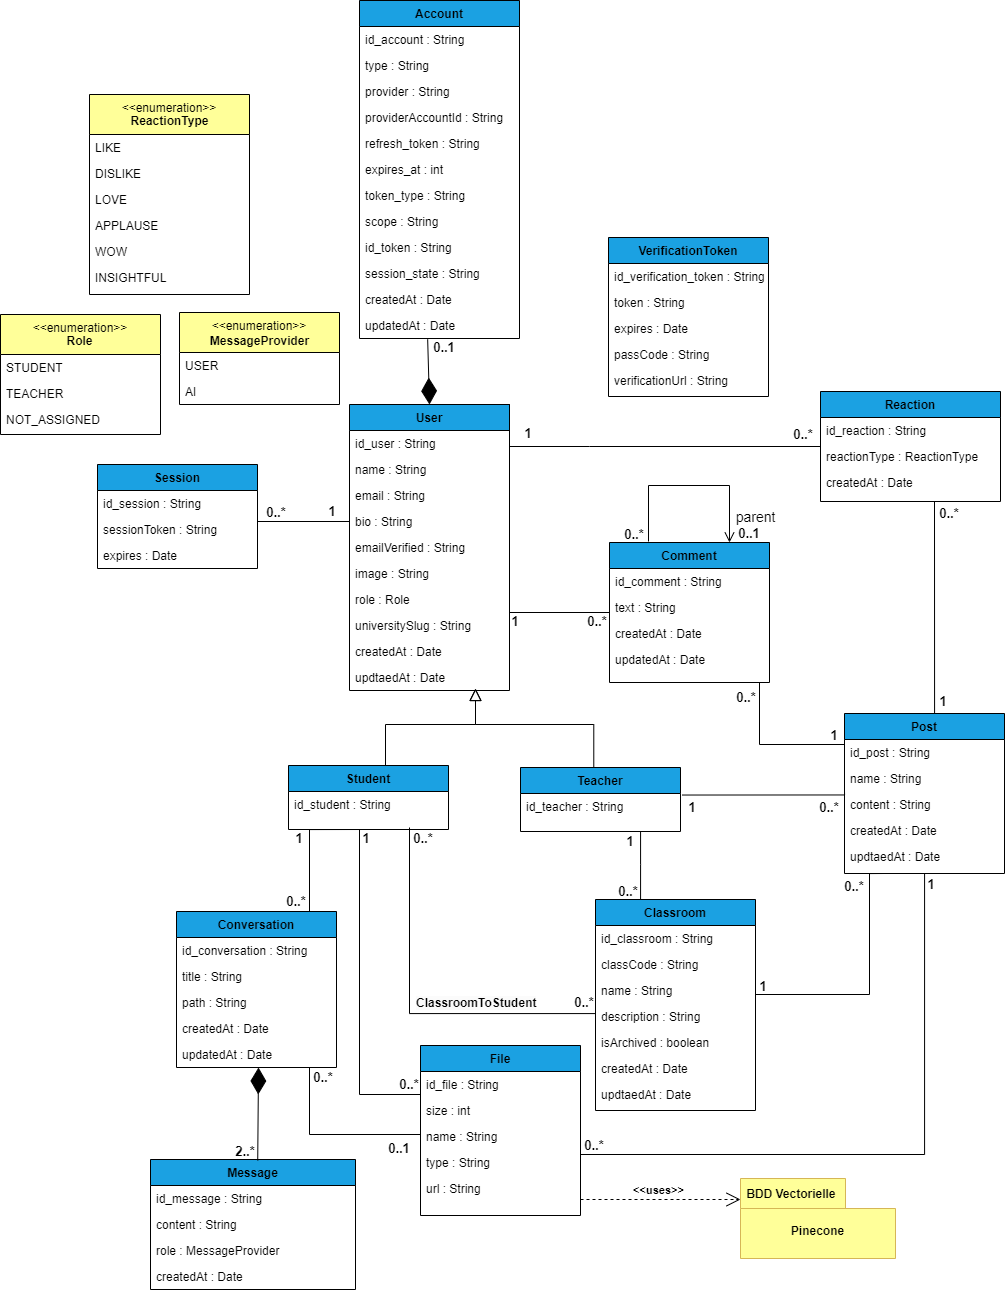
\includegraphics[width=1.1\textwidth,height=1.45\textwidth]{images/chp4/fig6.png}
    \caption{Diagramme de classes}
    \label{fig:Diagramme de classes}    
\end{figure}

\subsection{Conception de la vue dynamique}
La vue dynamique illustre la manière dont les éléments d'un système logiciel interagissent et se comportent en mettant l'accent sur les séquences d'actions et les échanges de messages entre eux.

\subsubsection{Diagramme de séquence de conception}
\justifying
Dans cette partie, nous mettons en évidence la progression des opérations et des échanges entre les différentes couches de l'application en utilisant des diagrammes de séquence de conception.
\begin{itemize}[itemsep=1pt, parsep=1pt]
    \newpage
    \item \textbf{Diagramme de séquence de conception « S’identifier » }\\
        La Figure 4.7 illustre le diagramme de séquence de conception \textbf{« S’identifier »} 
        \begin{figure}[H]
            \centering
            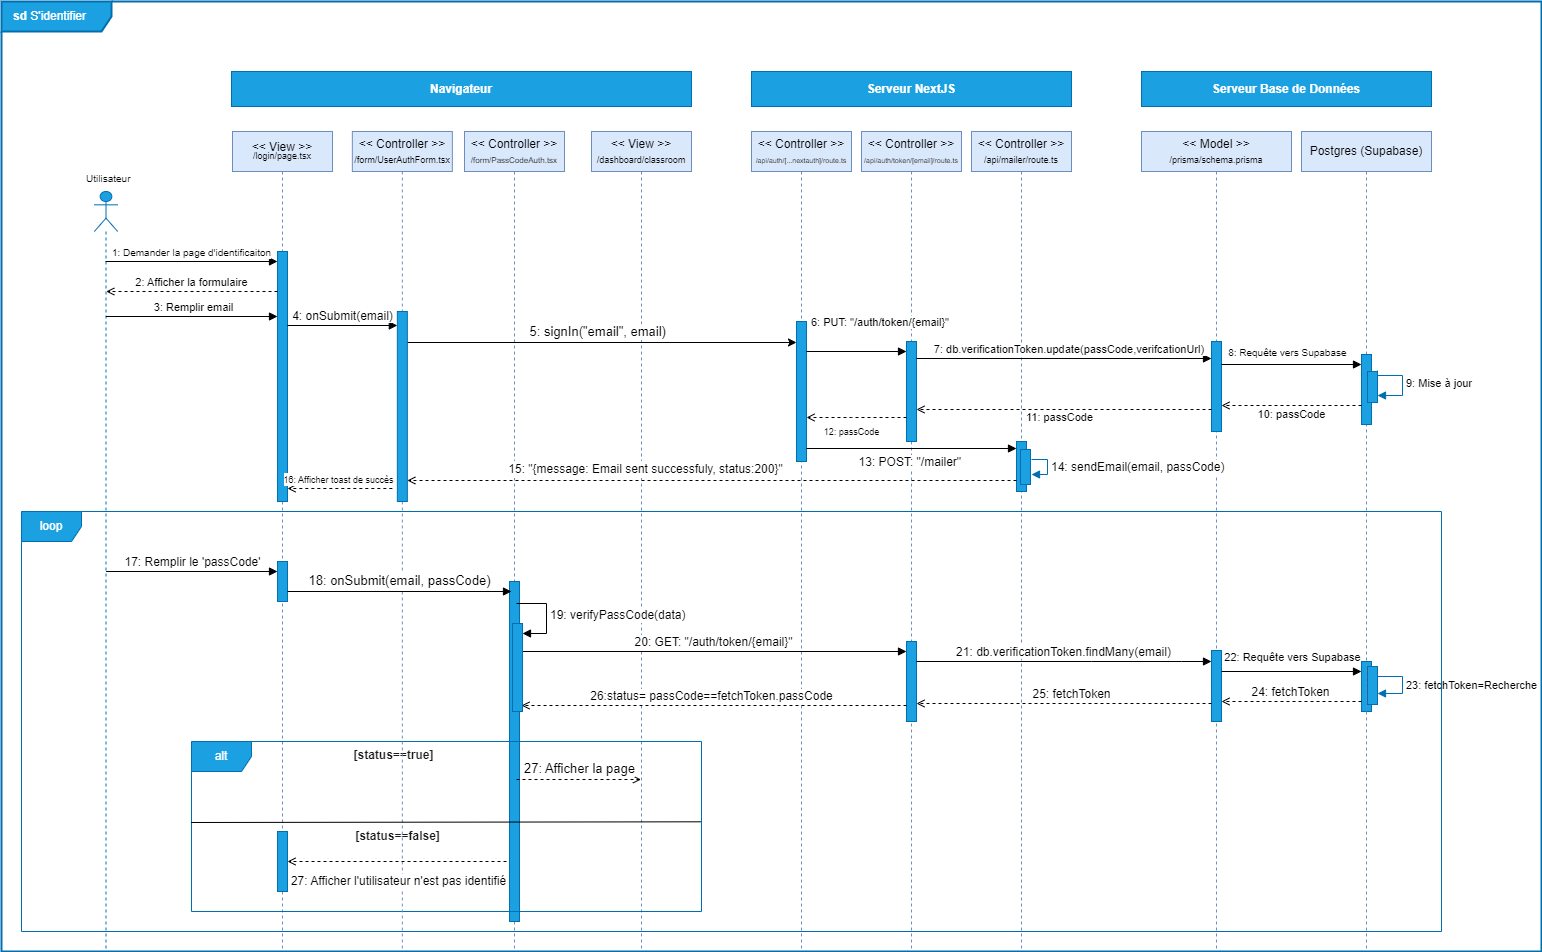
\includegraphics[width=1.32\textwidth,height=1\textwidth,angle=90]{images/chp4/fig7.png}
            \caption{Diagramme de séquence de conception « S’identifier »}
            \label{fig:Diagramme de séquence de conception « S’identifier »}    
        \end{figure}
    \item \textbf{Diagramme de séquence de conception « Créer classroom » }\\
        La Figure 4.8 illustre le diagramme de séquence de conception \textbf{« Créer classroom »} 
        \begin{figure}[H]
            \centering
            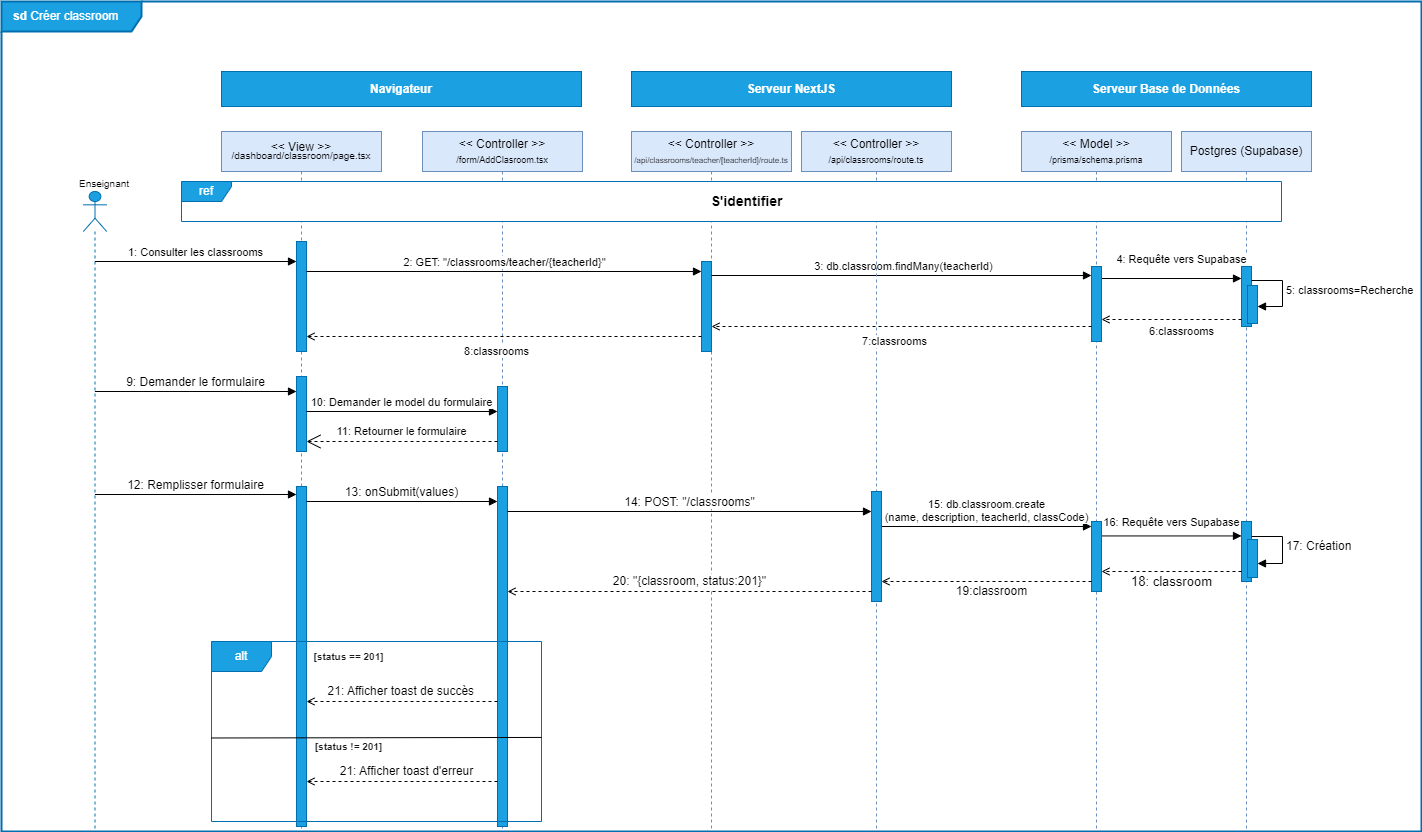
\includegraphics[width=1.32\textwidth,height=1\textwidth,angle=90]{images/chp4/fig8.png}
            \caption{Diagramme de séquence de conception « Créer classroom »}
            \label{fig:Diagramme de séquence de conception « Créer classroom »}    
        \end{figure}
    \item \textbf{Diagramme de séquence de conception « Démarrer chat »}\\
    La Figure 4.9 illustre le diagramme de séquence de conception \textbf{« Démarrer chat »} 
    \begin{figure}[H]
        \centering
        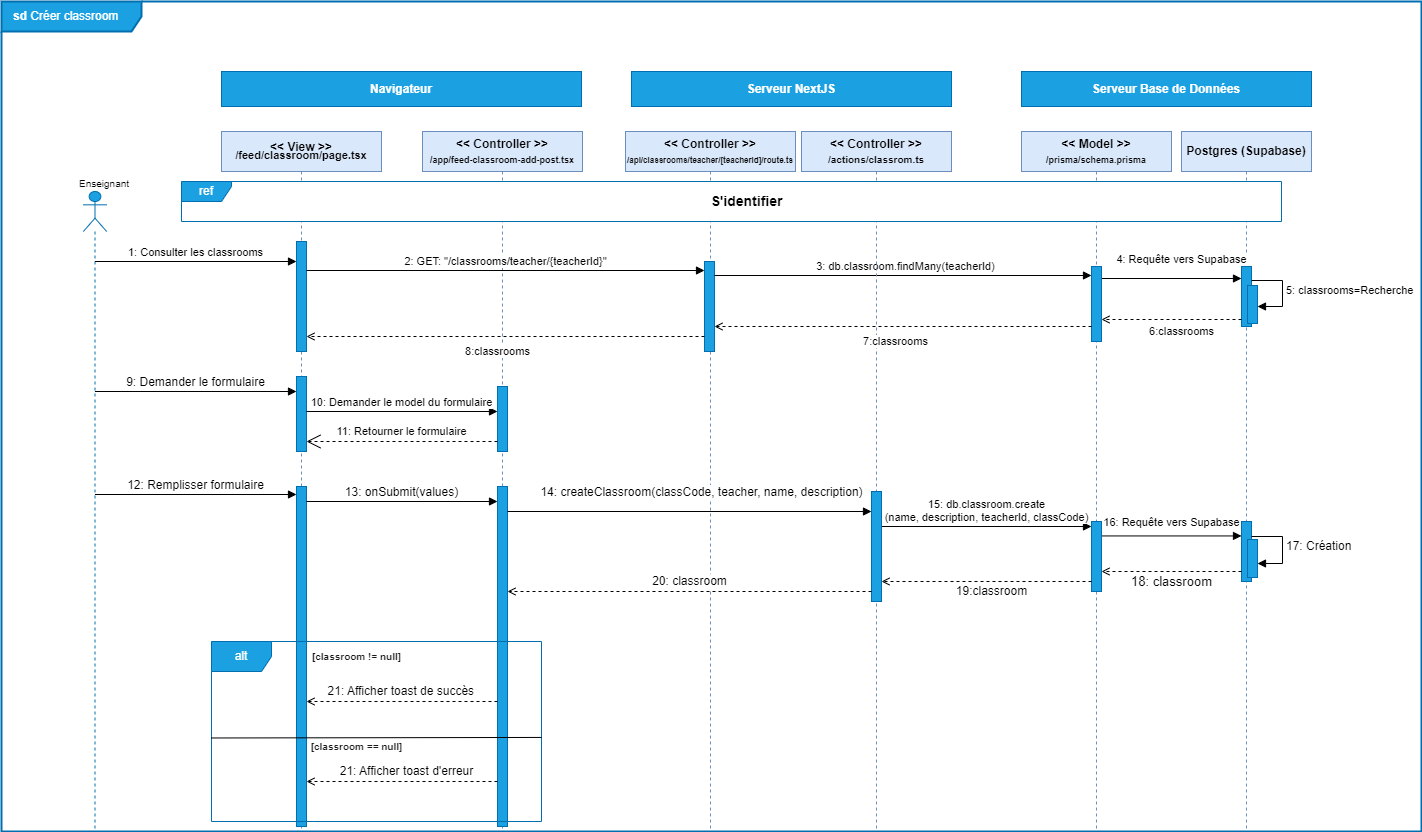
\includegraphics[width=1.32\textwidth,height=1\textwidth,angle=90]{images/chp4/fig9.png}
        \caption{Diagramme de séquence de conception « Démarrer chat »}
        \label{fig:Diagramme de séquence de conception « Démarrer chat »}    
    \end{figure}
\end{itemize}


\subsubsection{Diagramme d’activité « Modifier profil »}
\justifying
Le diagramme d'activité illustre le déroulement des opérations et des actions au sein d'un processus. Il offre la possibilité de représenter le processus séquentiel des étapes d'un système ainsi que les choix effectués à chaque étape. \\
La Figure 4.10 illustre le diagramme d’activité pour le cas d’utilisation \textbf{<< Modifier profil >>} sachant que l'utilisateur peut être soit un étudiant, soit un enseignant.

\begin{figure}[H]
    \centering
    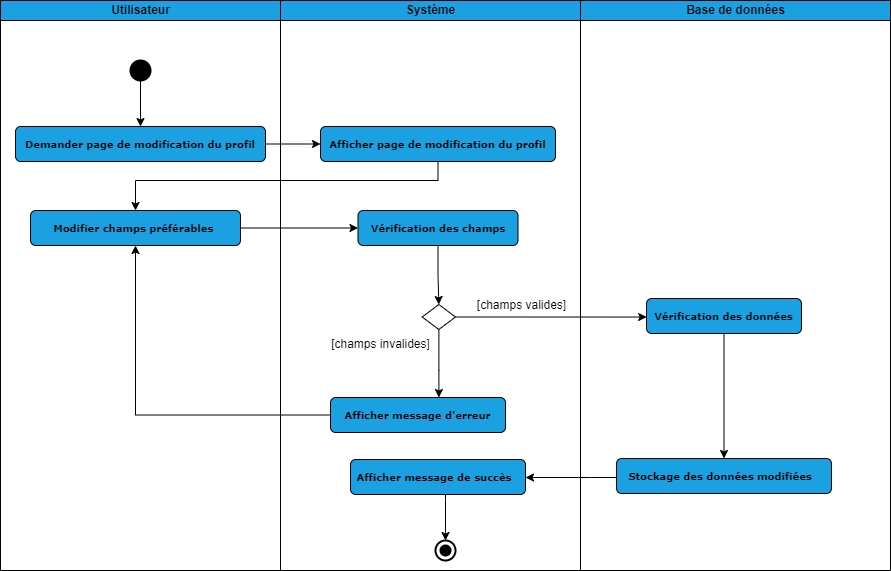
\includegraphics[width=\textwidth]{images/chp4/fig10.png}
    \caption{Diagramme d’activité « Modifier Profil »}
    \label{fig:Diagramme d’activité « Modifier Profil »}    
\end{figure}

\subsubsection{Diagramme d’états-transitions « Classroom »}
\justifying
Le diagramme d'états-transitions illustre les divers états d'un objet ou d'un système. Il permet de représenter les changements d’état qui peuvent se produire en réponse à des événements spécifiques.\\
La Figure 4.11 illustre le diagramme d’états-transitions de l’objet \textbf{<<Classroom>>} qui peut être  \textbf{<<désarchivé>>} ou  \textbf{<<archivé>>}.

\begin{figure}[H]
    \centering
    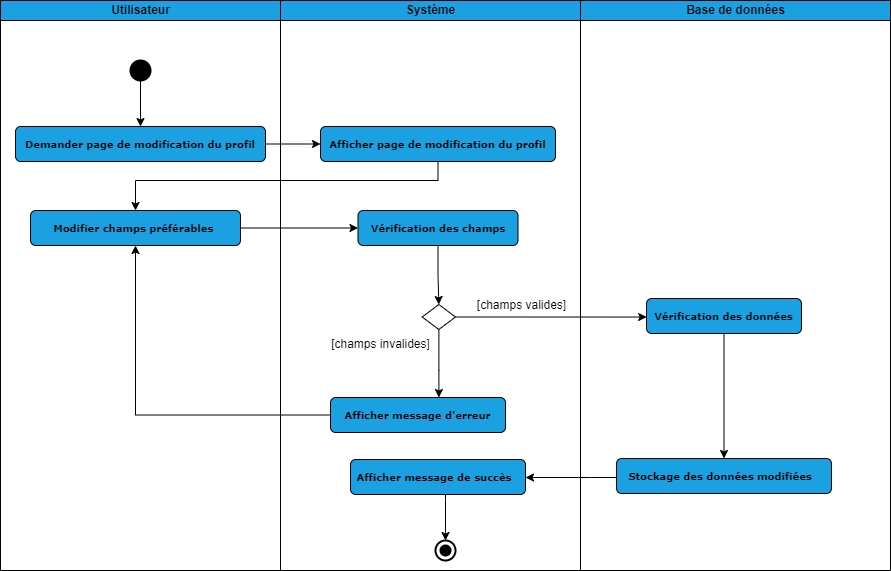
\includegraphics[width=\textwidth,height=0.28\textwidth]{images/chp4/fig11.png}
    \caption{Diagramme d’états-transitions d'objet « Classroom »}
    \label{fig:Diagramme d’états-transitions d'objet « Classroom »}    
\end{figure}

\subsubsection{Diagramme de timing}
Un diagramme de timing (temps) est un genre de diagrammes d'interaction qui est spécialement conçu pour prendre en compte les contraintes temporelles d'un logiciel.\\
Dans ce type de diagramme, les messages représentent les communications ou les interactions entre les différentes entités du système. Ils peuvent être synchrones, asynchrones ou des appels de méthodes. En plus, le diagramme de timing peut inclure aussi des informations sur les états des entités impliquées à des différents moments de l’exécution du système.\\
La Figure 4.12 illustre le diagramme de timing du cas d’utilisation \textbf{<< Démarrer chat >>} et plus spécifiquement lors de l’envoie d’un message.

\begin{figure}[H]
    \centering
    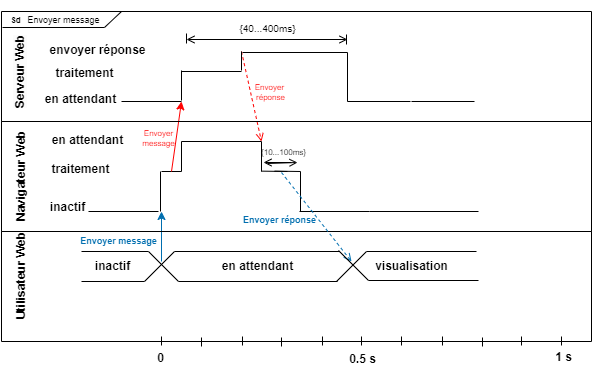
\includegraphics[width=\textwidth]{images/chp4/fig12.png}
    \caption{Diagramme de timing « Démarrer chat »}
    \label{fig:Diagramme de timing « Démarrer chat »}    
\end{figure}

\section{Conception graphique: Maquettage}
\justifying
La conception graphique, également appelée conception visuelle, joue un rôle essentiel dans la création de produits visuels tels que les sites web, les applications mobiles, les interfaces utilisateur, les affiches, les logos, les brochures (annonces) et d'autres éléments visuels.\\
Dans ce qui suit, nous allons présenter quelques exemples de maquettes de notre application afin de satisfaire les besoins et les expériences des utilisateurs sur une page spécifique.
\begin{itemize}
    \item \textbf{Maquette << Register Page >>}
\end{itemize}
La Figure 4.13 montre la maquette de l’interface \textbf{<< Register Page >>}
\begin{figure}[H]
    \centering
    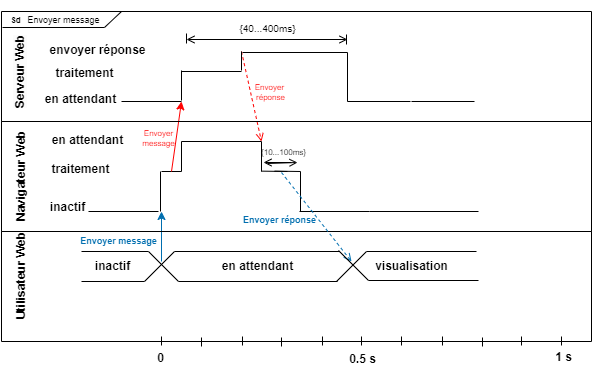
\includegraphics[width=0.85\textwidth,height=0.4\textwidth]{images/chp4/fig13.png}
    \caption{Maquette de l’interface << Register Page >>}
    \label{fig:Maquette de l’interface <<Register Page>>}    
\end{figure}
\begin{itemize}
    \item \textbf{Maquette << Classroom Page >>}
\end{itemize}
La Figure 4.14 montre la maquette de l’interface \textbf{<< Classroom Page >>}
\begin{figure}[H]
    \centering
    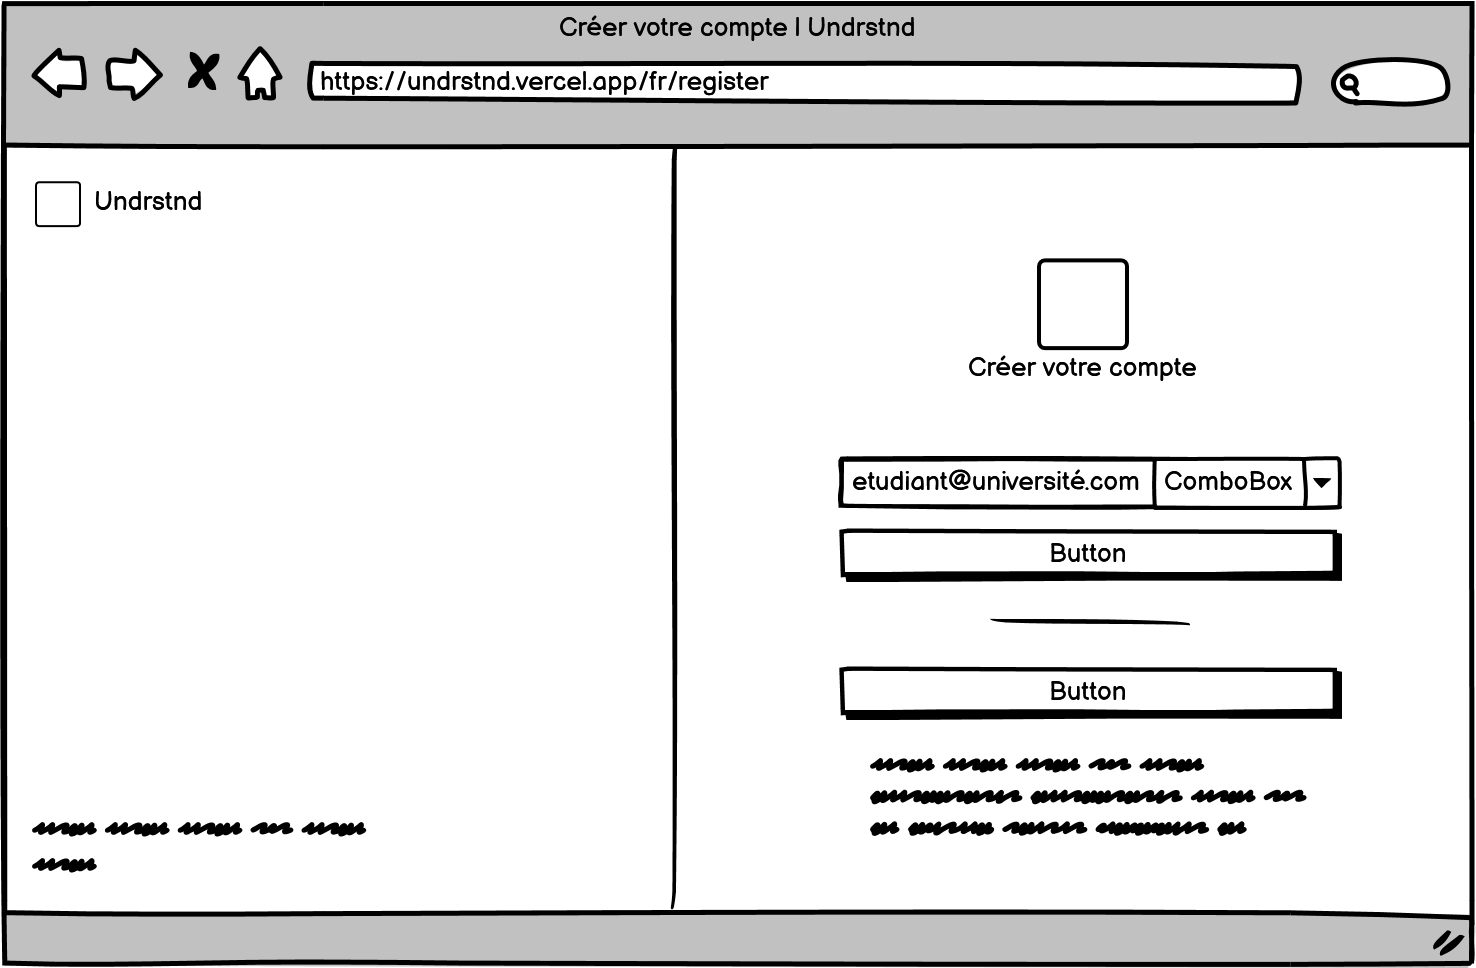
\includegraphics[width=0.85\textwidth,height=0.4\textwidth]{images/chp4/fig14.png}
    \caption{Maquette de l’interface << Classroom Page >>}
    \label{fig:Maquette de l’interface <<Classroom Page>>}    
\end{figure}
\begin{itemize}
    \item \textbf{Maquette <<Chat Page>>}
\end{itemize}
La Figure 4.15 montre la maquette de l’interface \textbf{<< Chat Page >>}
\begin{figure}[H]
    \centering
    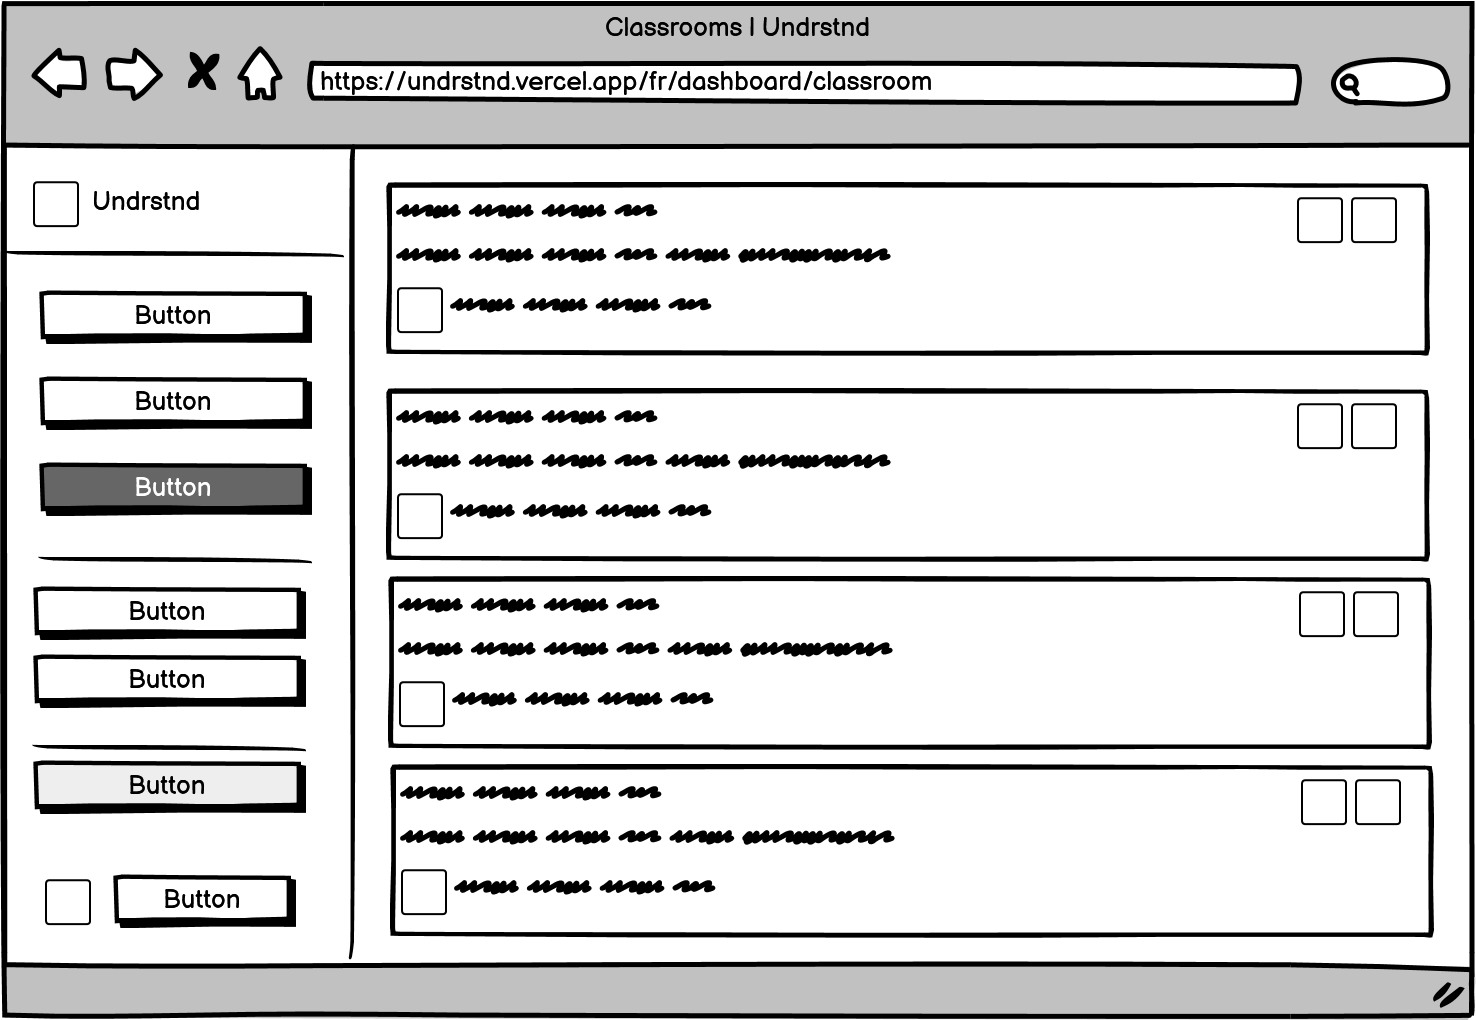
\includegraphics[width=0.85\textwidth,height=0.5\textwidth]{images/chp4/fig15.png}
    \caption{Maquette de l’interface << Chat Page >>}
    \label{fig:Maquette de l’interface <<Chat Page>>}    
\end{figure}
\begin{itemize}
    \item \textbf{Maquette << Chat Page with uploading File >>}
\end{itemize}
La Figure 4.16 montre la maquette de l’interface \textbf{ << Chat Page >>}, plus spécifiquement lors de l’importation d’un fichier.
\begin{figure}[H]
    \centering
    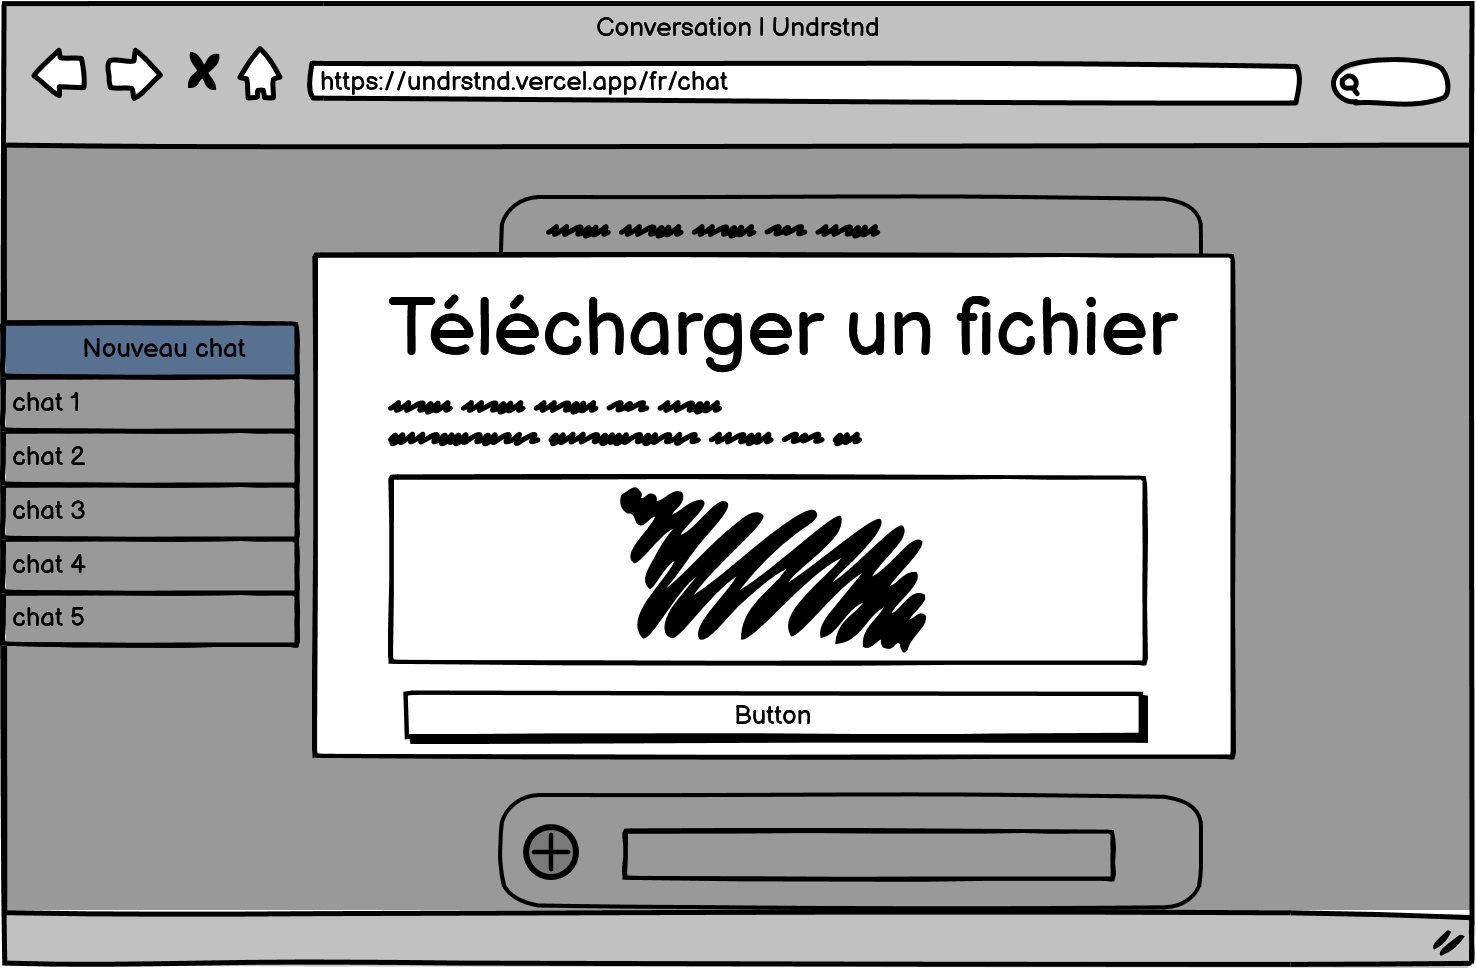
\includegraphics[width=0.85\textwidth,height=0.5\textwidth]{images/chp4/fig16.png}
    \caption{Maquette de l’interface << Chat Page with uploading File >>}
    \label{fig:Maquette de l’interface <<Chat Page with uploading File>>}    
\end{figure}
\section*{Conclusion}
Au cours de ce chapitre, nous avons exposé en détail les étapes clés de la conception de notre projet. En effet, nous avons commencé par la présentation de l’architecture de notre application. Puis, nous avons défini le modèle conceptuel et le modèle logique de notre base de données. Ensuite, nous avons exposé la conception logicielle de notre application en spécifiant la vue statique via le diagramme de classes et la vue dynamique via les diagrammes de séquence de conception, un diagramme d’activité, un diagramme d’états-transitions et un diagramme de timing. Enfin, nous avons présenté quelques maquettes pour la conception graphique. Le chapitre suivant sera consacré à détailler le reste du dernière branche, notamment la réalisation de notre plateforme.


